\documentclass[fullscreen=true,unicode,bookmarks=true]{beamer}

\usepackage{ofvp_beamer_packages} % Дополнительные пакеты для презентации и PDF для МЛЦ

\usepackage{ofvp_beamer_theme} % Тема презентаций для МЛЦ

\pretitle{Дипломная работа}
\title{Самофокусировка лазерных импульсов с~регулярной поперечной структурой и~сравнительный анализ филаментации на~длинах волн 0.8~и~10~мкм в воздухе}
\author[Ефимов О.\,В.]{Олег Ефимов}
\supervisorname{к.\,ф.-м.\,н. доцент С.\,А. Шлёнов}
\institute[МГУ имени М.\,В. Ломоносова]{
Московский государственный университет имени М.\,В. Ломоносова \\
Физический факультет \\
Кафедра Общей Физики и Волновых Процессов \\
}
\date[2010]{22 декабря 2010}

% PDF settings
\hypersetup{
	pdftitle={Дипломная работа},%
	pdfauthor={Ефимов О.В.},%
	pdfsubject={Самофокусировка лазерных импульсов с регулярной поперечной структурой и сравнительный анализ филаментации на длинах волн 0.8 и 10 мкм в воздухе},%
	pdfkeywords={диплом, филаментация, лазер, физика, оптика, вычислительные методы, параллельное программирование, самофокусировка, дифракция, дисперсия, уравнение квазиоптики, уравнение Шрёдингера}
}

% Root path for all images and graphs
\graphicspath{{../figures/}}

\begin{document}

    \begin{frame}
        \titlepage
    \end{frame}

	\section{Введение}

    \subsection{Проблема управления началом филаментации}

    \begin{frame}
        \frametitle{Проблема управления началом филаментации}

		\begin{columns}[c,totalwidth=\textwidth]
			\column[c]{0.7\textwidth}	
				Одними из приложений явления филаментации является
				FIBS-спектроскопия (filament induced breakdown spectroscopy).
		        Для FIBS важно уметь управлять расстоянием филаментации.
                Это~возможно сделать с~помощью временной или~пространственной модуляции импульса.

			\column[c]{0.3\textwidth}				
	        		\begin{figure}
	           			\includegraphics[width=0.8\textwidth]{slides_images/fibs}
	        		\end{figure}
		\end{columns}
    \end{frame}

    \subsection{Изменение характеристик филамента при разных длинах волн}

    \begin{frame}
        \frametitle{Изменение характеристик филамента на разных длинах волн лазерного излучения}

		В ряде последних работ по филаментации лазерного излучения в~воздухе
		исследуется изменение характеристик филамента
		($I^{fil}$, $N_e^{fil}$, $r_{fil}$, $r_{pl}$) в зависимости от длины волны излучения.
		На данный момент экспериментально и численно исследована филаментация
		на длинах волн в диапазоне 248--1240 нм.
		
		\vfill		
		
        [1] \textit{В.Ю. Фёдоров.}
		Влияние параметров фемтосекундного лазерного импульса на филаментацию в атмосфере /
		Кандидатская диссертация. Физический факультет МГУ им. М.\,В. Ломоносова.— 2010.
    \end{frame}

    \subsection{Цели работы}

    \begin{frame}
        \frametitle{Цели работы}

        \begin{enumerate}
			\item Анализ самофокусировки лазерных импульсов с регулярной поперечной структурой.
			      Исследование различных режимов филаментации в зависимости от мощности пучка
			      и разности фаз в соседних элементах структуры.
			\item Численное моделирование процесса филаментации излучения $CO_2$-лазера в воздухе.
			      Сравнительный анализ филаментации на~длинах волн 800~нм и 10~мкм.
		\end{enumerate}
    \end{frame}

    \section{Физическая модель и численные методы}

	\subsection{Математическая модель}

    \begin{frame}
        \frametitle{Математическая модель филаментации}
		
        Уравнение медленно меняющейся амплитуды:
        \begin{equation*}
        	2ik\frac{\partial E}{\partial z} =
        	\Delta_{\perp}E -
        	k\frac{\partial^2 k}{\partial \omega^2}\frac{\partial E^2}{\partial t^2} + 
        	\frac{2k^2}{n_0}\left[ \Delta n_k + \Delta n_p \right] E  - i k \alpha E
        \end{equation*}

		Керровская нелинейность:
        \begin{equation*}
			\Delta n_k(\vec{r}, z, t) = n_2 I(\vec{r}, z, t)
		\end{equation*}
		
		Плазменная нелинейность:
        \begin{equation*}
			\Delta n_p(\vec{r}, z, t) = -\frac{\omega_p^2}{2 n_0 \omega_0^2}
		\end{equation*}
		
		Уравнение динамики плотности электронов:
        \begin{equation*}
			\dfrac{\partial N_{e}^{(N_2,O_2)}}{\partial t} = R_{\lambda}(I)\left(N_{0}^{(N_2,O_2)} - N_{e}^{(N_2,O_2)}\right)
		\end{equation*}
    \end{frame}
    
	\section{Самофокусировка пучков с регулярной поперечной структурой}
	
    \begin{frame}
        \frametitle{Самофокусировка пучков с регулярной поперечной структурой}

        Периодический пучки с гауссовой огибающей:
        \begin{eqnarray*}
          	E^{outphase}(x, y, z = 0) & = & E_0 \exp\left( -\frac{x^2+y^2}{2 r_0^2} \right) \cos(\alpha_m x) \cos(\alpha_m y) \\
           	E^{inphase}(x, y, z = 0) & = & E_0 \exp\left( -\frac{x^2+y^2}{2 r_0^2} \right) \left| \cos(\alpha_m x) \cos(\alpha_m y) \right|
        \end{eqnarray*}

		\vspace{-2em}

        \begin{figure}[H]
            \begin{center}
                \begin{minipage}[h]{0.4\linewidth}
                    \center{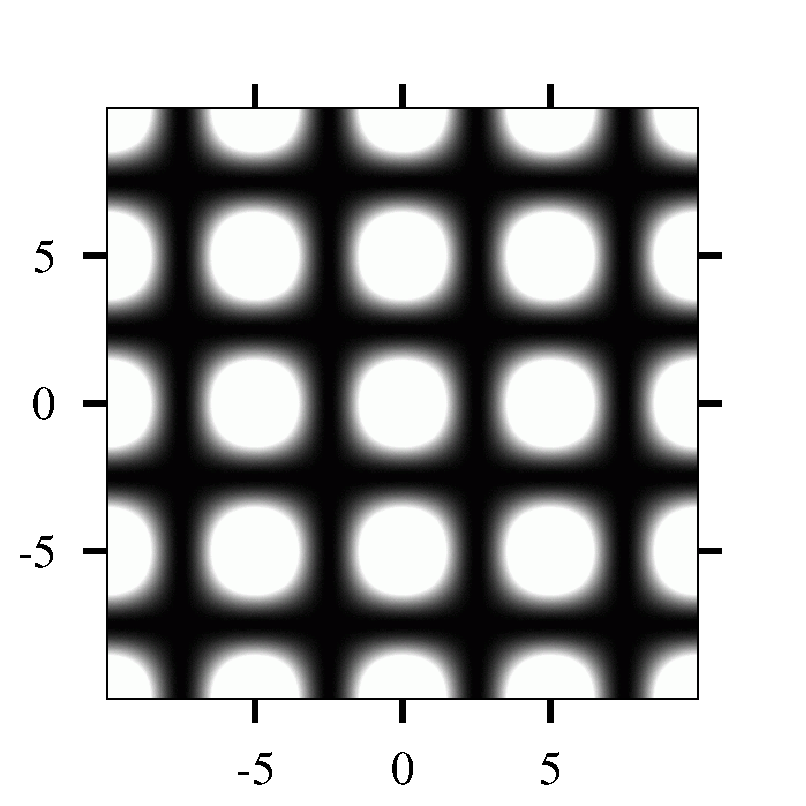
\includegraphics[width=0.95\linewidth]{beams/r_1000/out00000_norm}}
                \end{minipage}
            \end{center}
        \end{figure}
    \end{frame}	

    \begin{frame}
        \frametitle{Режим с образованием множества филаментов: $P_{1}/P_{cr}^{Gauss} \approx 2$}

        \begin{figure}[H]
            \begin{center}
                \begin{minipage}[h]{0.49\linewidth}
                    \center{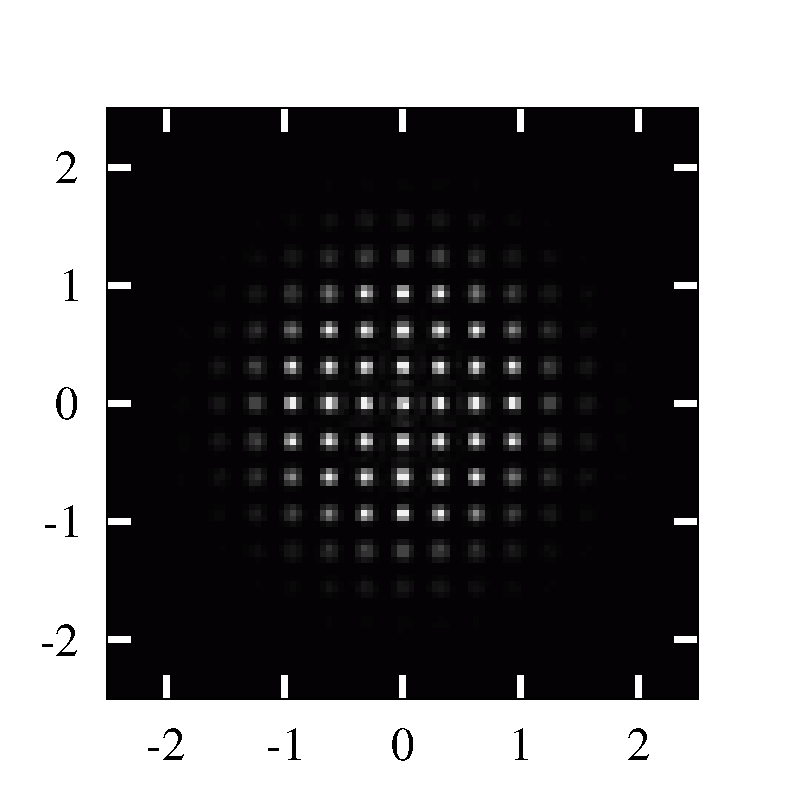
\includegraphics[width=0.95\linewidth]{beams/r_1000/outphase_norm}} \\ Противофазная \\ модуляция
                \end{minipage}
                \hfill
                \begin{minipage}[h]{0.49\linewidth}
                    \center{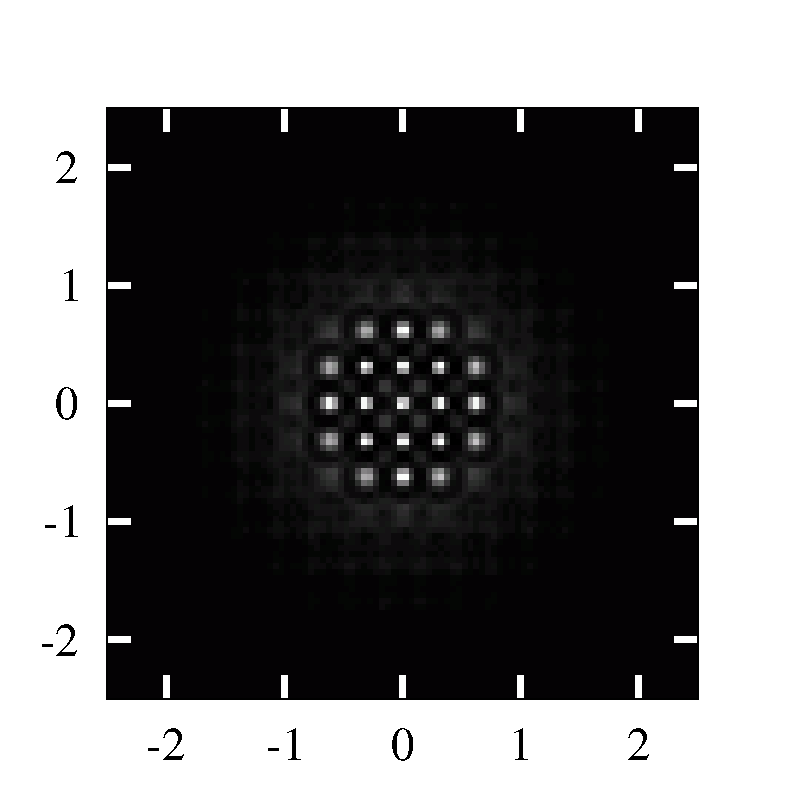
\includegraphics[width=0.95\linewidth]{beams/r_1000/inphase_norm}} \\ Синфазная \\ модуляция
                \end{minipage}
            \end{center}
        \end{figure}
    \end{frame}

    \begin{frame}
        \frametitle{Процесс филаментации пучка с регулярной поперечной структурой при~$P/P_{cr}^{Gauss} = 13.3$}
        	
        	Синфазный пучок:
        	\vspace{-1em}
            \begin{figure}[H]
                \begin{center}
                    \begin{minipage}[h]{0.24\linewidth}
                        \center{\includegraphics[width=\linewidth]{slides_images/r_50_inphase/out00100_norm}} \\ \footnotesize{$z = 0.1$} \\
                    \end{minipage}
                    \hfill
                    \begin{minipage}[h]{0.24\linewidth}
                        \center{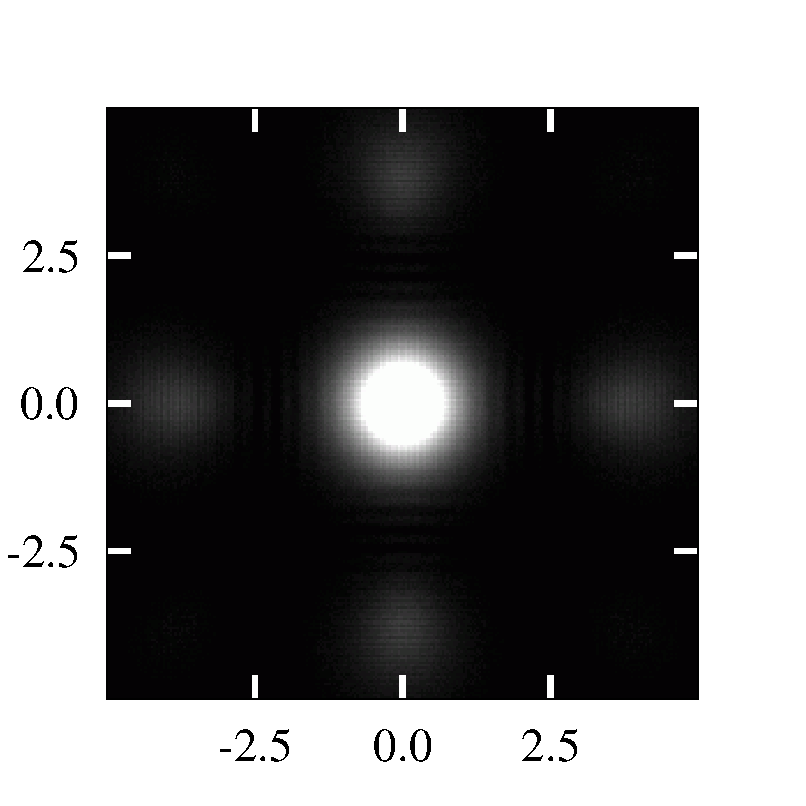
\includegraphics[width=\linewidth]{slides_images/r_50_inphase/out00200_norm}} \\ \footnotesize{$z = 0.2$} \\
                    \end{minipage}
                    \hfill
                    \begin{minipage}[h]{0.24\linewidth}
                        \center{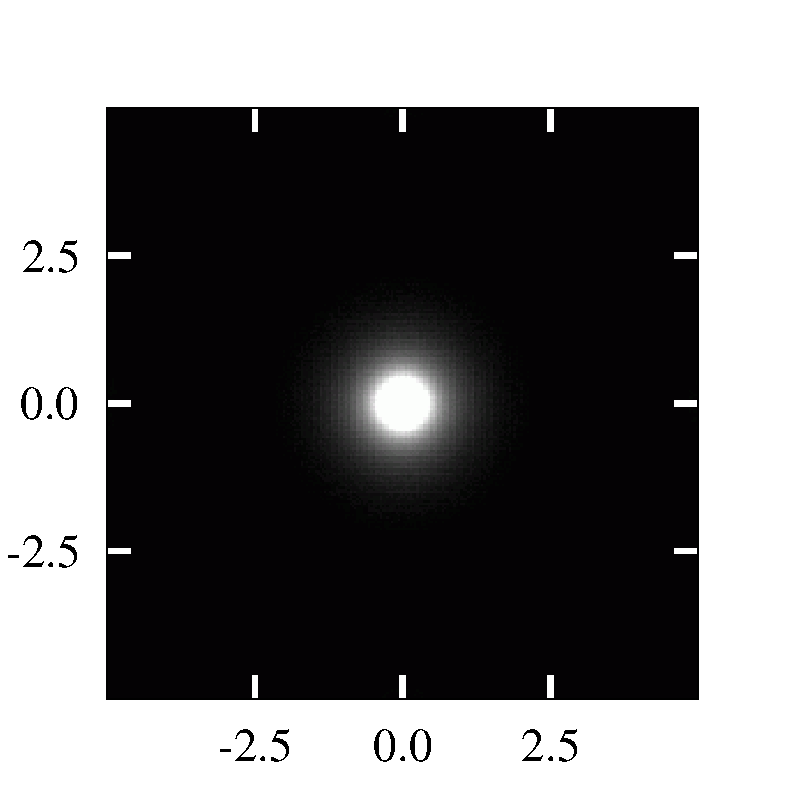
\includegraphics[width=\linewidth]{slides_images/r_50_inphase/out00300_norm}} \\ \footnotesize{$z = 0.3$} \\
                    \end{minipage}
                    \hfill
                    \begin{minipage}[h]{0.24\linewidth}
                        \center{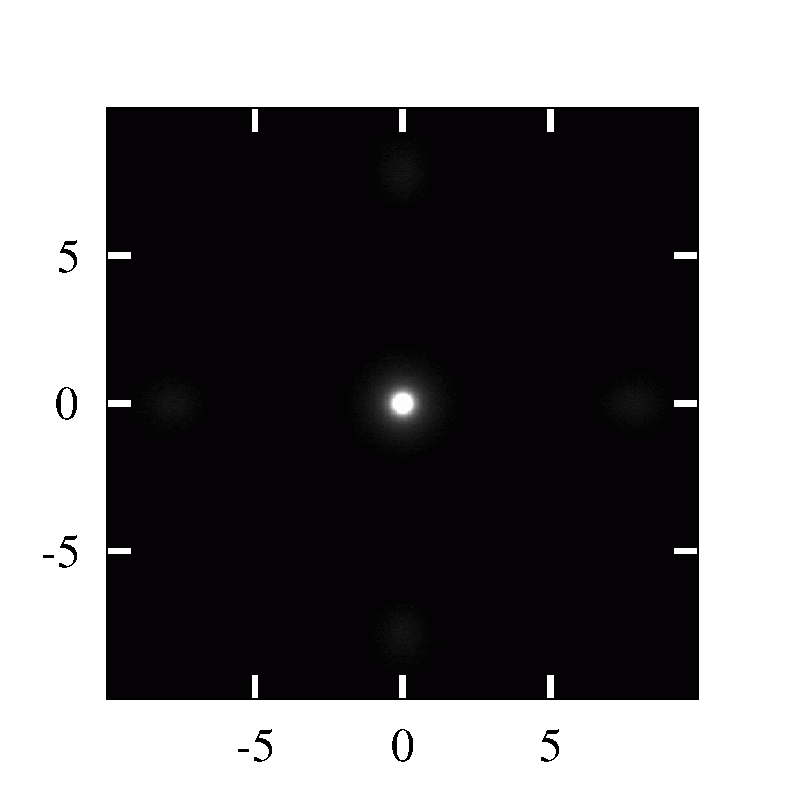
\includegraphics[width=\linewidth]{slides_images/r_50_inphase/out00400_norm}} \\ \footnotesize{$z = 0.4$} \\
                    \end{minipage}
                \end{center}
            \end{figure}

			Противофазный пучок:
			\vspace{-1em}
            \begin{figure}[H]
                \begin{center}
                    \begin{minipage}[h]{0.24\linewidth}
                        \center{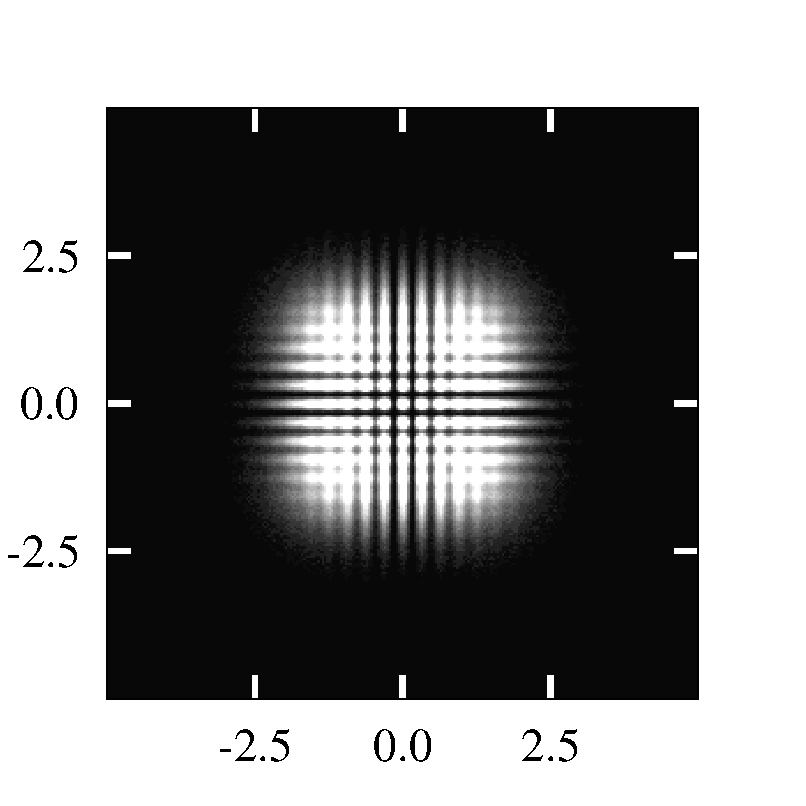
\includegraphics[width=\linewidth]{slides_images/r_50_outphase/out00010_norm}} \\ \footnotesize{$z=0.1$} \\
                    \end{minipage}
                    \hfill
                    \begin{minipage}[h]{0.24\linewidth}
                        \center{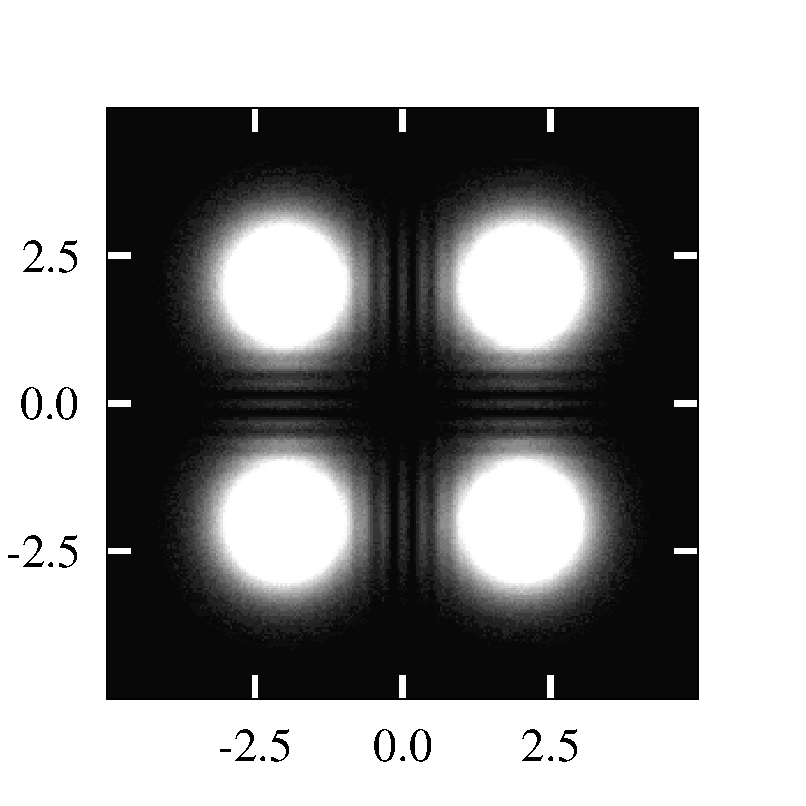
\includegraphics[width=\linewidth]{slides_images/r_50_outphase/out00020_norm}} \\ \footnotesize{$z=0.2$} \\
                    \end{minipage}
                    \hfill
                    \begin{minipage}[h]{0.24\linewidth}
                        \center{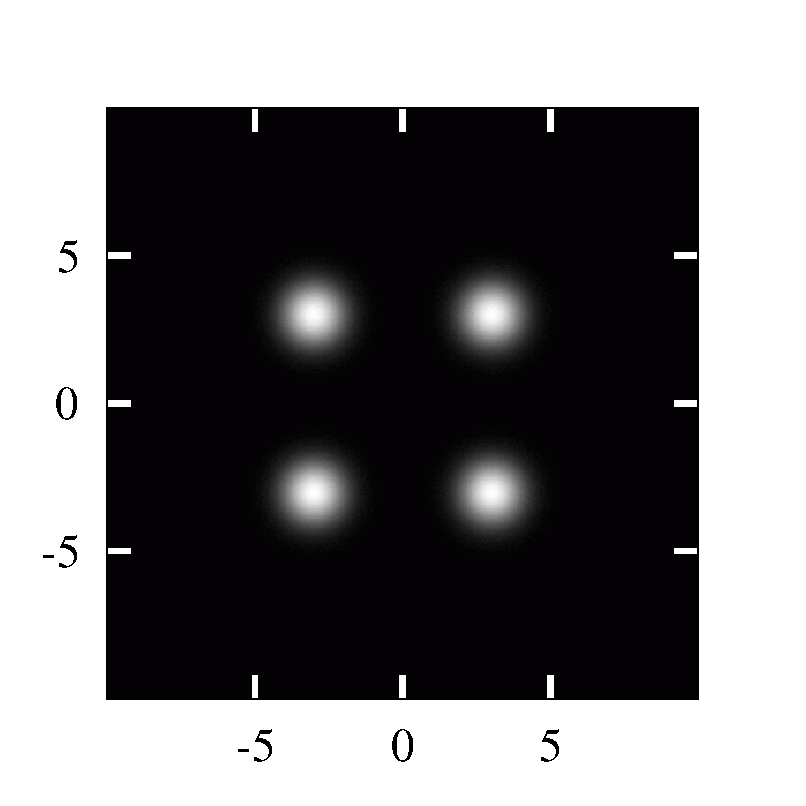
\includegraphics[width=\linewidth]{slides_images/r_50_outphase/out00030_norm}} \\ \footnotesize{$z=0.3$} \\
                    \end{minipage}
                    \hfill
                    \begin{minipage}[h]{0.24\linewidth}
                        \center{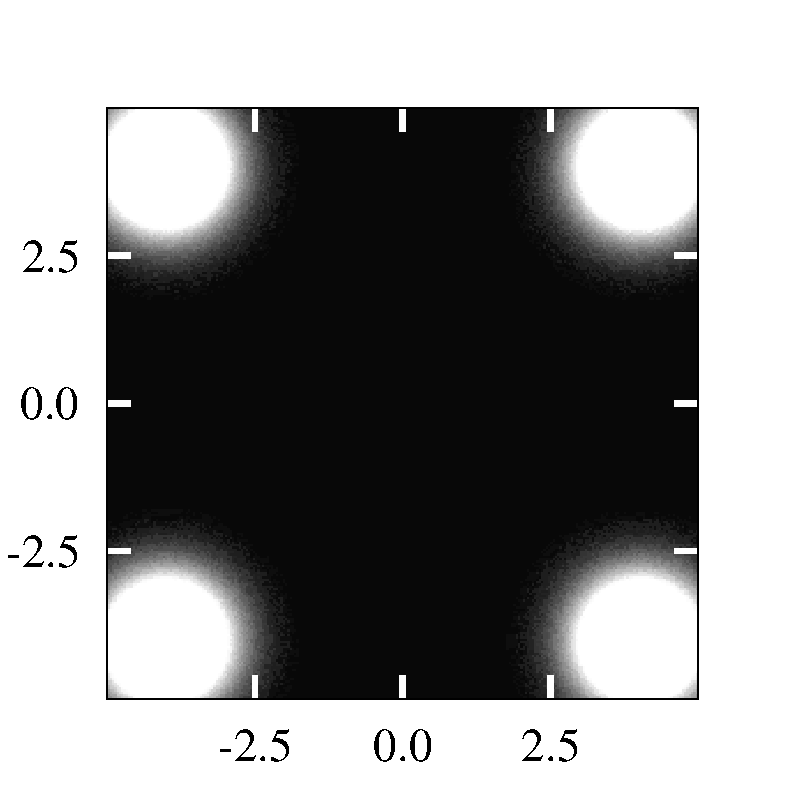
\includegraphics[width=\linewidth]{slides_images/r_50_outphase/out00040_norm}} \\ \footnotesize{$z=0.4$} \\
                    \end{minipage}
                \end{center}
            \end{figure}
    \end{frame}

    \begin{frame}
        \frametitle{Процесс филаментации противофазного пучка при~$P/P_{cr}^{Gauss} = 26.5$}

            \begin{figure}[H]
                \begin{center}
                    \begin{minipage}[h]{0.24\linewidth}
                        \center{\includegraphics[width=\linewidth]{slides_images/r_100_outphase/out00100_norm}} \\ \footnotesize{$z=0.1$} \\
                    \end{minipage}
                    \hfill
                    \begin{minipage}[h]{0.24\linewidth}
                        \center{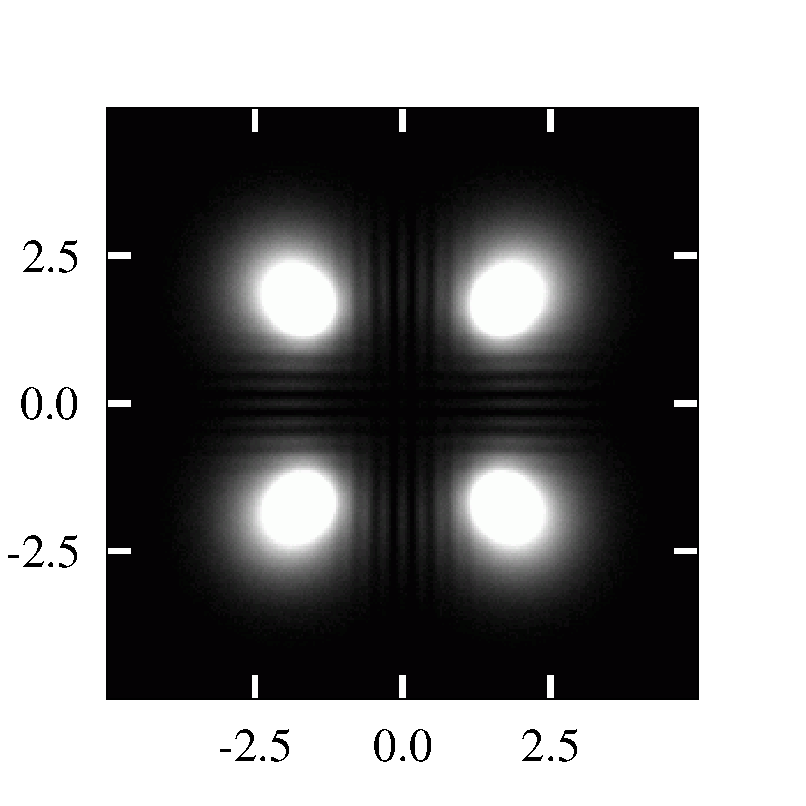
\includegraphics[width=\linewidth]{slides_images/r_100_outphase/out00200_norm}} \\ \footnotesize{$z=0.2$} \\
                    \end{minipage}
                    \hfill
                    \begin{minipage}[h]{0.24\linewidth}
                        \center{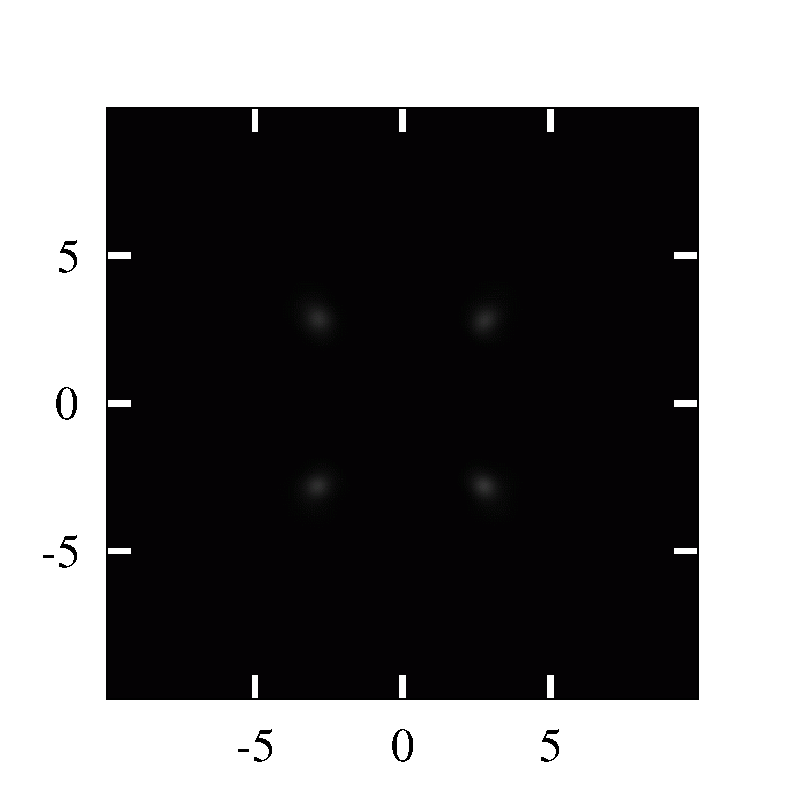
\includegraphics[width=\linewidth]{slides_images/r_100_outphase/out00300_norm}} \\ \footnotesize{$z=0.3$} \\
                    \end{minipage}
                    \hfill
                    \begin{minipage}[h]{0.24\linewidth}
                        \center{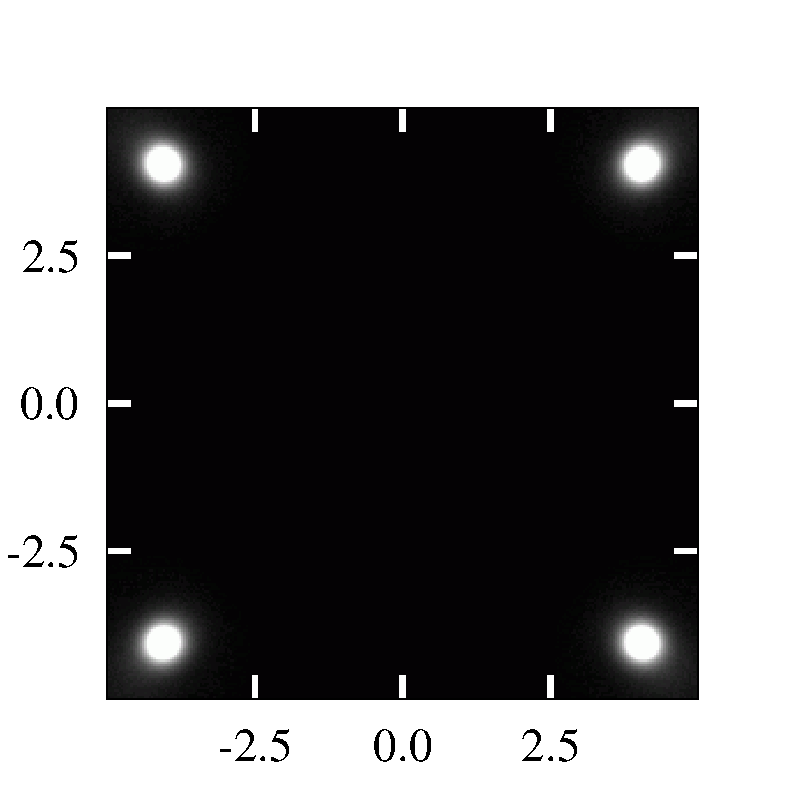
\includegraphics[width=\linewidth]{slides_images/r_100_outphase/out00400_norm}} \\ \footnotesize{$z=0.4$} \\
                    \end{minipage}
                \end{center}
            \end{figure}
    \end{frame}

	\subsection{Характер самофокусировки синфазного и противофазного пучков одинаковой мощности}

    \begin{frame}
        \frametitle{Характер самофокусировки синфазного и~противофазного пучков одинаковой мощности}

        \begin{figure}
        	\center{
        		\includegraphics[height=0.6\pdfpageheight]{slides_images/beams_intensity_comparison/graph_all} \\
        		{\small Зависимость пиковой интенсивности от расстояния.}
        	}
        \end{figure}
    \end{frame}

    \begin{frame}
        \frametitle{Особенности начального этапа распространения синфазного и~противофазного пучков одинаковой мощности}

	        \begin{figure}
	        	\center{
	        		\includegraphics[height=0.6\pdfpageheight]{slides_images/beams_intensity_comparison/graph_start} \\
	        		{\small Зависимость пиковой интенсивности от расстояния.}
	        	}
	        \end{figure}
    \end{frame}

    \begin{frame}
        \frametitle{Режим однофиламентации синфазного пучка при ~$P/P_{cr}^{Gauss} = 26.5$}

            \begin{center}
                \movie[height=0.7\pdfpageheight,width=0.7\pdfpageheight,poster,showcontrols=true]{}{../figures/slides_video/inphase.avi}
            \end{center}
    \end{frame}

    \section{Изменение характеристик филамента при~разных~длинах~волн}

    \begin{frame}
        \frametitle{Постановка нестационарной задачи в осесимметричном приближении}

            Уравнение распространения в безразмерных цилиндрических координатах:
			\begin{equation*}
			2 i \dfrac{\partial E}{\partial z} = \dfrac{1}{r}\dfrac{\partial}{\partial r}\left(r\dfrac{\partial E}{\partial r}\right)
			- \dfrac{L_{diff}}{L_{disp}} \dfrac{\partial^2 E}{\partial t^2} + R |E|^2 E - R_{I} N_{e} E - i \alpha E
			\end{equation*}

            Начальные условия:
			\begin{equation*}\label{PulsesInitialConditions}
			E(\vec{r}, z = 0, t) = E_0 \cdot \exp\left(-\frac{r^2}{2 r_0^2}\right) \cdot \exp\left(-\frac{t^2}{2 \tau_0^2}\right)
			\end{equation*}
			
			При этом скорость ионизации $R_{\lambda=800}(I)$ рассчитана по~модели~ППТ, а~$R_{\lambda=10000}(I)$ --- по~модели~АДК.
    \end{frame}	

    \begin{frame}
        \frametitle{\small{Сравнение полученных характеристик филамента и~плазменного канала
                    при~филаментации излучения на~длинах волн 800~нм и 10~мкм}}

        \begin{figure}[H]
            \begin{center}
                \begin{minipage}[h]{0.40\linewidth}
                    \includegraphics[width=0.95\linewidth]{pulses/vs/intensity_cut}
                \end{minipage}
                \hspace{0.10\linewidth}
                \begin{minipage}[h]{0.40\linewidth}
                    \includegraphics[width=0.95\linewidth]{pulses/vs/plasma_cut}
                \end{minipage}
                \\
                \begin{minipage}[h]{0.40\linewidth}
                    \includegraphics[width=0.95\linewidth]{pulses/vs/r_fil_cut}
                \end{minipage}
                \hspace{0.10\linewidth}
                \begin{minipage}[h]{0.40\linewidth}
                    \includegraphics[width=0.95\linewidth]{pulses/vs/r_pl_cut}
                \end{minipage}
            \end{center}
        \end{figure}
        
        \footnotesize{
        	Параметры импульсов: $2 r_0(\lambda_{800}) = 0.25$~см, $2 r_0(\lambda_{10000}) = 0.88$~см, $L_{diff} = 12.2$~м,
        	$2\tau_0 = 750$~фс, $P/P_{cr} = 1.5$.
        }
    \end{frame}

    \begin{frame}
        \frametitle{\small{Сравнение полученных характеристик филамента и~плазменного канала
                    при~филаментации излучения на~длинах волн 800~нм и 10~мкм}}
       	
		\begin{tabular*}{\linewidth}{@{\extracolsep{\fill}} c c c c c c c }
		\toprule
		$\lambda$ & $z_{fil}$, м & $I_{fil}, \textsf{ Вт}/\textsf{см}^2$ & $N_e^{fil}, \textsf{ см}^{-3}$ & $r_{fil}, \textsf{ мкм}$   & $r_{pl}, \textsf{ мкм}$ \\
		\midrule
		10 мкм    & 11.52        & $2.12 \cdot 10^{13}$                  & $0.01 \cdot 10^{16}$           & 839                        & 198                     \\
		800 нм    & 11.77        & $8.91 \cdot 10^{13}$                  & $4.4 \cdot 10^{16}$            & 38.2                       & 8.8                     \\
		\bottomrule
		\end{tabular*}

		\begin{columns}[c,totalwidth=\textwidth]
			\column[c]{0.4\textwidth}	
				\onslide<2>{
				\begin{figure}[H]
				    \begin{center}
				        \begin{minipage}[h]{\linewidth}
				            \center{\includegraphics[width=0.95\linewidth]{pulses/comparison/slides_plasma}} \\
				            {\small Пиковая концентрация плазмы}
				        \end{minipage}
				    \end{center}
				\end{figure}
				}

			\column[c]{0.2\textwidth}				
				\begin{eqnarray*}
					N_e^{fil}(\lambda) & \sim & \frac{1}{\lambda^2} \\
					r_{fil} & \sim & \lambda \\
					r_{pl} & \sim & \lambda
				\end{eqnarray*}

			\column[c]{0.4\textwidth}	
				\onslide<2>{			
				\begin{figure}[H]
				    \begin{center}
				        \begin{minipage}[h]{\linewidth}
				            \center{\includegraphics[width=0.95\linewidth]{pulses/comparison/slides_r_pl}} \\
				            {\small Радиус плазменного канала}
				        \end{minipage}
				    \end{center}
				\end{figure}
				}
		\end{columns}
    \end{frame}

	\section{Выводы}

	\begin{frame}
		\frametitle{Выводы I}
		
        \begin{enumerate}
			\item Исследована филаментация гауссового пучка с регулярной поперечной структурой
                  и различными фазовыми соотношениями между соседними элементами этой структуры.
			\item Показано, что при одинаковых остальных параметрах в случае синфазной модуляции
                  образуется один филамент, а в случае противофазной модуляции
                  возникает четыре филамента, разбегающиеся от оси распространения исходного
                  импульса, и~вследствие этого в случае противофазного пучка критическая
                  мощность самофокусировки примерно в 4 раза больше, чем~в~синфазном случае.
                  Таким образом, существует область значений мощности пучка, при которой
                  в синфазном случае филамент образуется, а в противофазном --- нет.
		\end{enumerate}
	\end{frame}
	
	\begin{frame}
		\frametitle{Выводы II}
		
        \begin{enumerate}
			\item Рассмотрена одиночная филаментация осесимметричного импульса
			      и разработана расчётная программа,
			      учитывающая дифракцию, керровскую нелинейность, дисперсию второго порядка и ионизацию
			      с учётом раздельной концентрации ионов кислорода и азота в воздухе.
			\item Проведено сравнение характеристик возникающего филамента и~плазменного канала при филаментации излучения
			      на длинах волн 800 нм и 10 мкм для двух импульсов с одинаковыми длительностями, дифракционной длиной
			      и превышением пиковой мощности над критической мощностью самофокусировки.
			\item Показано, что при увеличении длины волны излучения диаметр филамента и плазменного канала увеличиваются,
			      тогда как концентрация плазмы уменьшается. Характеристики филаментов, получаемых при самофокусировке излучения
			      на длине волны 10~мкм, успешно описываются зависимостями, полученными из~обобщения экспериментов
			      по~филаментации излучения видимого и ближнего ИК диапазонов.
		\end{enumerate}
	\end{frame}	

\end{document}
